\documentclass[12pt, a4paper]{report}
\setcounter{secnumdepth}{0}
\usepackage{graphicx}
\usepackage{titlesec}
\usepackage{pdfpages}
\usepackage{wrapfig}
\usepackage[T1]{fontenc}
\usepackage[utf8]{inputenc}
\graphicspath{ {./images/} }

\title{
  \begin{huge}
    \textbf{
      {Computer Science Project 2020-'21}\\
      {Sudoku Web App}
    }\\
  \end{huge}
  \begin{figure}
      \centering
      {
\includegraphics[scale=2]{iss}}
  \end{figure}
}
\author{
x % add only one name here
}

\date{\vspace{-5ex}}

\begin{document}

  \begin{titlepage}
  \maketitle
  \end{titlepage}

  \newpage
  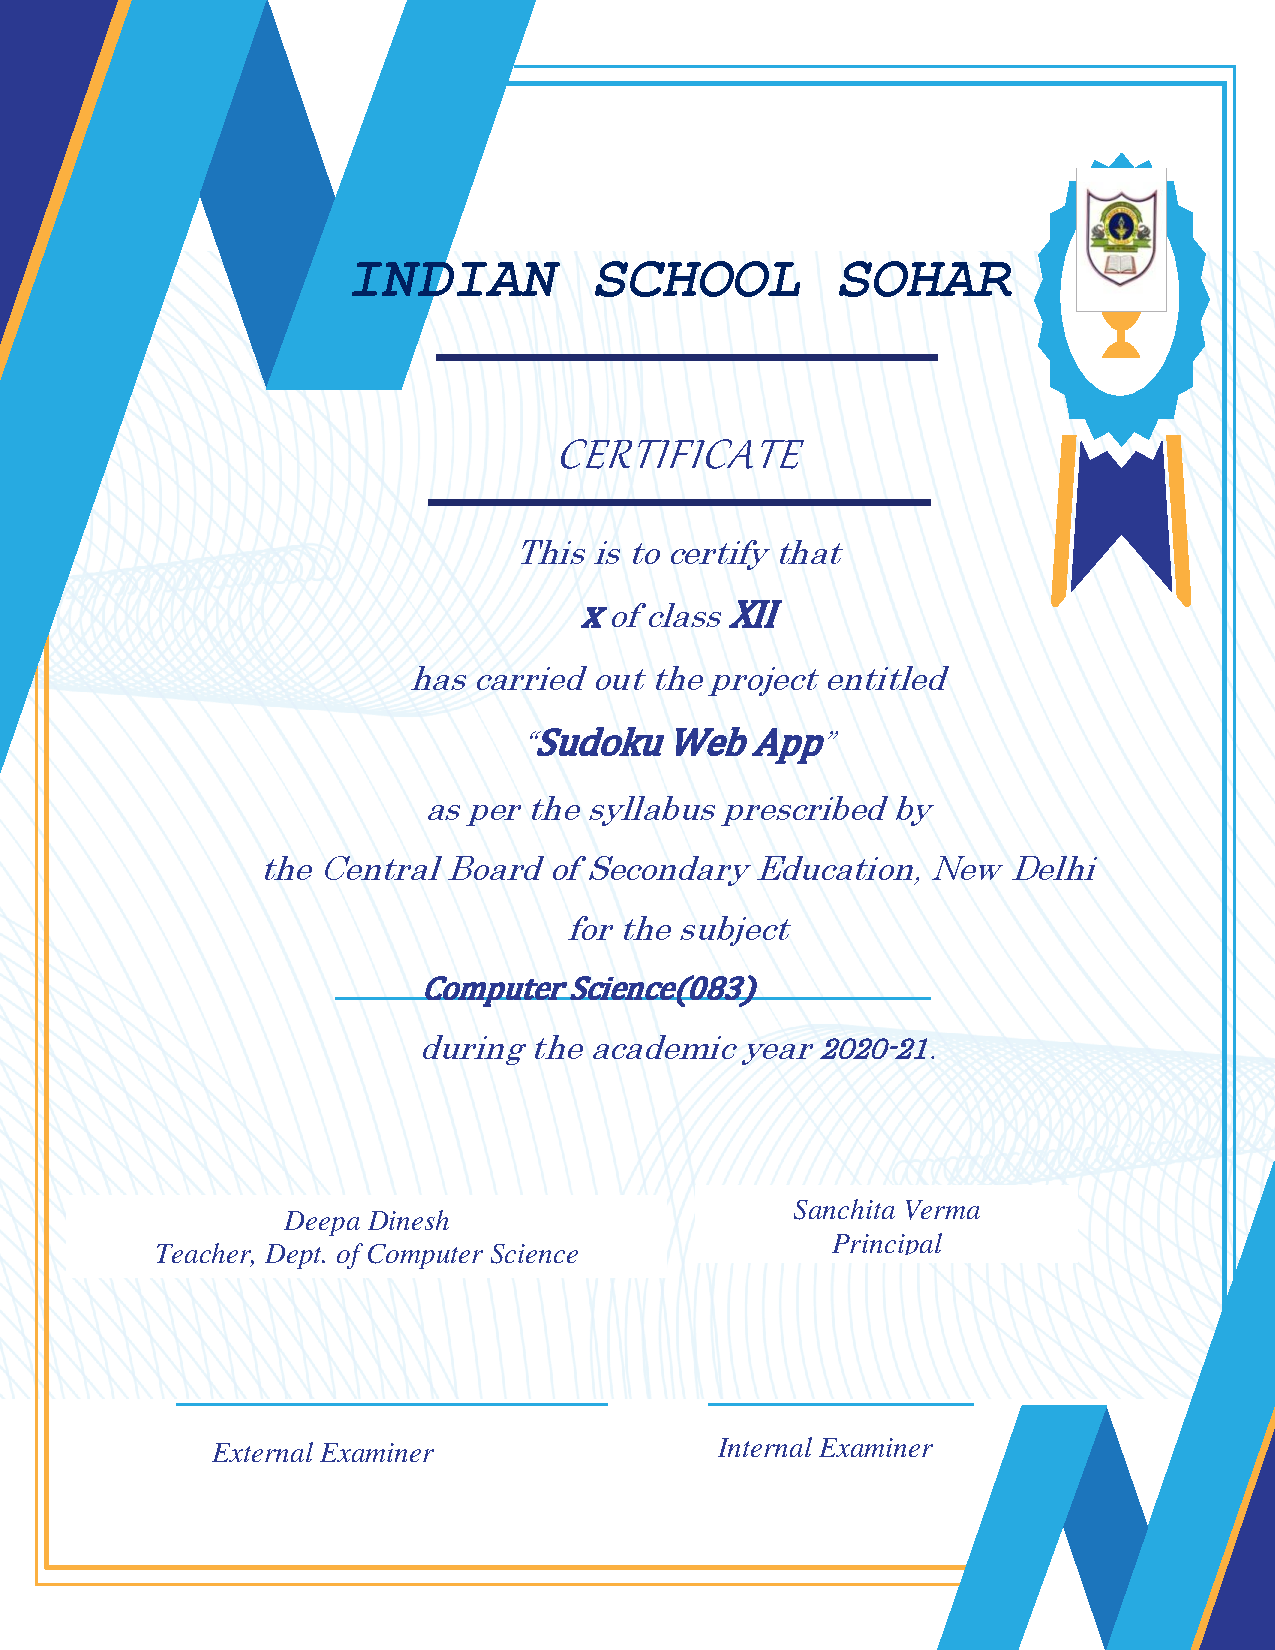
\includepdf{cert}
  
  \newpage
  \maketitle
  \begin{large}
  \section*{Acknowledgements}
  I have taken efforts in this project. However, it would not have been possible without the kind support and help of many individuals and organizations. I would like to extend my sincere thanks to all of them. \newline
  \newline
  I am greatly indebted to the teacher-in-charge, Ms.~Deepa Dinesh for her guidance and constant supervision as well as for providing necessary information 
  regarding the project and also for her support in completing the project. \newline
  \newline
  I would like to express my gratitude towards my parents for their kind cooperation and encouragement which helped me in the completion of this project. \newline
  \newline
  I would also like to express my special gratitude and thanks to my classmates in developing the project and to the people who have willingly 
  helped me out with their abilities.
  \end{large}
 
  \maketitle
  \begin{large}
  \newpage
  \tableofcontents
  \end{large}
  
  \newpage
  \section{Introduction}
  Python was created in the late 1980s, and first released in 1991, by Guido van Rossum as a successor to the ABC programming language.
  \begin{wrapfigure}{r}{0.25\textwidth}
    
\includegraphics[width=0.25\textwidth]{introduction}
  \end{wrapfigure}
  Python is an interpreted, object-oriented, high-level programming language with dynamic semantics. Its high-level built in data structures, combined with dynamic typing and dynamic binding, make it very attractive for Rapid Application Development, as well as for use as a scripting or glue language to connect existing components together.

  Python's simple, easy to learn syntax emphasizes readability and therefore reduces the cost of program maintenance. Python supports modules and packages, which encourages program modularity and code reuse. The Python interpreter and the extensive standard library are available in source or binary form without charge for all major platforms, and can be freely distributed.
  
  \subsection{Features in Python:}
    \subsubsection{Easy to code:}
    Python is a high-level programming language. Python is very easy to learn as compared to other languages like C, C#, JavaScript, Java, etc. It is very easy to code in python language and anybody can learn python basics in a few hours or days. It is also a developer-friendly language.
    
    \subsubsection{Free and Open Source:}
    Since it is open-source, this means that source code is also available to the public. So you can download it as, use it as well as share it.
    
    \subsubsection{Object-Oriented Language:}
    One of the key features of Python is Object-Oriented Programming. Python supports object-oriented language and concepts of classes, objects, encapsulation, etc.
    
    \subsubsection{High-Level Language:}
    Python is a high-level language. When we write programs in Python, we do not need to remember the system architecture or manage memory.
    
  \newpage
  \section{Feasibility Study}
   The feasibility study is the important step in any software development process. This is because it makes analysis of different aspects like - cost required for developing and executing the system, the time required for each phase of the system and so on. If these important factors are not analyzed then definitely it would have impact on the organization & the development and the system would be a total failure.

  The purpose of feasibility study is not to solve the problem, but to determine whether the problem is worth solving. By making analysis this way it would be possible to make a report of identified area of problem. By making a detailed analysis in this area a detailed document or report is prepared in this phase which has details like project plan or schedule of the project, the cost estimated for developing and executing the system, target dates for each phase of delivery of system developed and so on. This phase is the base of software development process since further steps taken in software development life cycle would be based on the analysis made on this phase and so careful analysis has to be made in this phase.
  
  \subsection{TELOS}
  
    The feasibility study concentrates on the following area (TELOS):
    \begin{itemize}
      \item Technology and System Feasibility
      \item Economic Feasibility
      \item Legal Feasibility
      \item Operational Feasibility
      \item Schedule Feasibility
    \end{itemize}
  
    \subsubsection{Technology and System Feasibility}
    The assessment is based on an outline design of system requirements, to determine whether the company has the technical expertise to handle completion of the project. Economic feasibility (Cost/Benefit Analysis)
  
    \subsubsection{Economic Feasibility}
    The economic feasibility study evaluates the cost of the software development against the ultimate income or benefits expected from the developed system. It includes identifying cost and benefit factors like - Development costs and Operating costs. There must be scopes for profit after the successful completion of the project.
  
    \subsubsection{Legal Feasibility}
    It determines whether the proposed system conflicts with legal requirements, e.g. a data processing system must comply with the local Data Protection Acts.
  
    \subsubsection{Operational Feasibility}
    Operational feasibility is a measure of how well a proposed system solves the problems, and takes advantage of the opportunities identified during scope definition and how it satisfies the requirements identified in the requirements analysis phase of system development.
  
    \subsubsection{Schedule Feasibility}
    A project will fail if it takes too long to be completed before it is useful. Typically this means estimating how long the system will take to develop, and if it can be completed in a given time period using some methods like payback period. Schedule feasibility is a measure of how reasonable the project timetable is. Given our technical expertise, are the project deadlines reasonable?
    
  \subsection{Advantages of Feasibility Study}
    \begin{itemize}
      \item As the initial step of software development life cycle, feasibility study has all the analysis part in it, which helps in analyzing the system requirements completely. 
      \item Helps in identifying the risk factors involved in developing and deploying the system.
      \item It helps in making cost/benefit analysis which helps the organization and system to run efficiently.
      \item It is a report which could be used by the senior or top persons in the organization. This is because, based on the report the organization decides about cost estimation, funding and other important decisions which is very essential for an organization to run profitably and for the system to run stable.
    \end{itemize}
    
  \subsection{Software Development Life Cycle}
  The Systems Development Life Cycle (SDLC) is a conceptual model used in project management that describes the stages involved in an information system development project from an initial feasibility study through maintenance of the completed application. \newline
  \begin{wrapfigure}{r}{0.25\textwidth}
    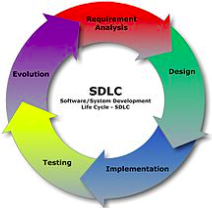
\includegraphics[width=0.25\textwidth]{feasibility-study}
  \end{wrapfigure}
  The following are the activities of the SDLC:
  \begin{itemize}
      \item Software requirement analysis
      \item Systems analysis and design
      \item Design/Code generation
      \item Testing
      \item Development and Maintenance
  \end{itemize}
  A Systems Development Life Cycle (SDLC) adheres to important phases that are essential for developers, such as planning, analysis, design, and implementation. A number of system development life cycle (SDLC) models have been created such as waterfall, fountain, spiral etc.
  
  \subsubsection{Requirement Analysis/Investigation}
  The 1st stage of SDLC is the investigation phase. During this stage, business opportunities and problems are identified, and information technology solutions are discussed. Multiple alternative projects may be suggested and their feasibility analyzed. The results of the feasibility study can then be compiled into a report, along with preliminary specifications. When the investigation stage ends, a decision whether or not to move forward with the project should be made.
  
  \subsubsection{System Analysis}
  The goal of system analysis is to determine where the problem is, in an attempt to fix the system. It analyzes the requirement for the proposed system. To understand the nature of the program to build, the system engineer must understand the information domain for the software, as well as required functions, performance and the interfacing. This step involves breaking down the system in different pieces to analyze the situation, analyzing project goals, breaking down what needs to be created. From the available information the system engineer develops a list of system level requirement for the project.
  
  \subsubsection{Design}
  Systems design describes screen layouts, business rules, process diagrams, a complete entity- relationship diagram with a full data dictionary and other documentation. It defines specifically how the software is to be written including an object model, the client/server technology, a detailed database design etc. These design elements are intended to describe the software in sufficient detail that skilled programmers may develop the software with minimal additional input design. Analysis and design are very important in the whole development cycle. Any glitch in the design could be very expensive to solve in the later stage of the software development. The design must be translated into a machine readable form.
  
  \subsubsection{Testing}
  In this stage, all the pieces of software are brought together into a special testing environment and then are checked for errors, bugs and interoperability. Unit, system and user acceptance testing is often performed.
  
  \subsubsection{Deployment and Maintenance}
  Deployment is the final stage of initial development. It involves installation, initial training and may involve hardware and network upgrades. Software will definitely undergo change once it is delivered to the customer. There may be many reasons for the change. Change could be due to some unexpected input values into the system. The software should be developed to accommodate changes that could take place during the post implementation period. Maintaining the system is also an important aspect of SDLC.
  
  
  \newpage
  \section{Hardware and Software}
   Add stuff here
  
  \newpage
  \section{About the Project}
  About the project
  
  \newpage
  \section{Source Code}
  Add a code overview here.
  
  \newpage
  \section{Bibliography}
  Add final output result here.
  
\end{document}
